\chapter{Estado del Arte}\label{chapter:state-of-the-art}

\section{Introduccion de RL}\label{section:state-of-the-art:introduction-to-RL}

La idea de aprender interactuando con el entorno es probablemente lo primero que se piensa cuando se habla de la naturaleza del aprendizaje. Cuando un bebé juega, agita los brazos o mira a su alrededor, no tiene un maestro explícito, pero sí una conexión sensorio motora directa con su entorno. El ejercicio de esta conexión produce una gran cantidad de información sobre la causa y el efecto, sobre las consecuencias de las acciones y sobre lo que hay que hacer para alcanzar los objetivos. A lo largo de su vida, estas interacciones son, sin duda, una importante fuente de conocimiento sobre el entorno y sobre ellos mismos. Tanto si aprenden a conducir un coche como a mantener una conversación, son conscientes de cómo responde el entorno a lo que hacen, y tratan de influir en lo que ocurre a través de su comportamiento. El aprendizaje a partir de la interacción es una idea fundamental que subyace en casi todas las teorías del aprendizaje y la inteligencia y cualquier método que se adapte bien a la resolución de este tipo de problemas lo se considera un método de aprendizaje por refuerzo.

En inteligencia artificial la tarea básica del aprendizaje por refuerzo consiste en capturar los aspectos más importantes del problema al que se enfrenta un agente que interactúa con su entorno para lograr un objetivo. Está claro que un agente de este tipo debe ser capaz de percibir el estado del entorno hasta cierto punto y debe ser capaz de realizar acciones que afecten al estado. El agente también debe tener uno o varios objetivos relacionados con el estado del entorno. Los problemas de aprendizaje por refuerzo implican aprender qué hacer, o sea cómo asignar situaciones a acciones, para maximizar una señal de recompensa numérica. En esencia, se trata de problemas de bucle cerrado porque las acciones del sistema de aprendizaje influyen en sus entradas posteriores. Además, no se le dice al agente qué acciones debe tomar, como en muchas formas de aprendizaje automático, sino que debe descubrir qué acciones producen la mayor recompensa al probarlas. En los casos más interesantes y desafiantes, las acciones pueden afectar no sólo a la recompensa inmediata, sino también a la siguiente situación y, a través de ella, a todas las recompensas posteriores. (\cite{sutton1998introduction})

\begin{figure}[ht!]
    \centering
    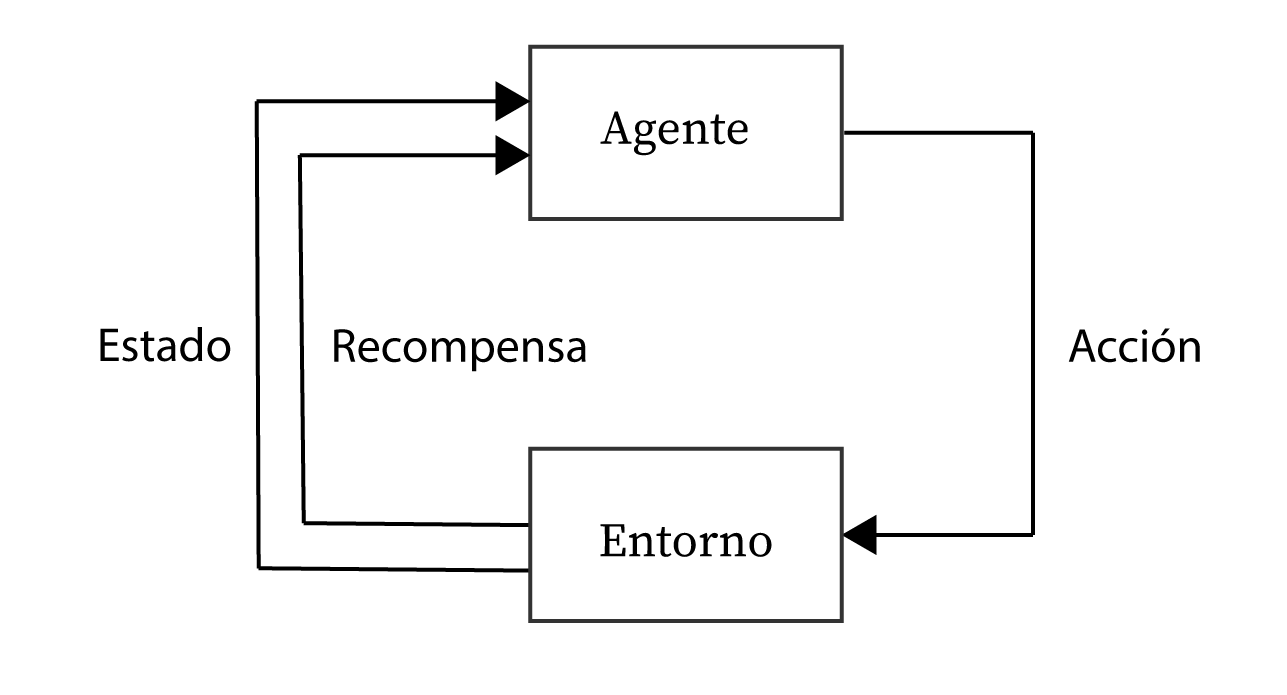
\includegraphics[width=0.7\textwidth]{Graphics/rl-elements.png}
    \caption{Diagrama de los componentes elementales del aprendizaje por refuerzo.}
    \label{fig:rl-elements}
\end{figure}

\subsection{Componentes del aprendizaje por refuerzo}

Más allá de los macro conceptos de agente, entorno, observaciones y acciones (Fig. \ref{fig:rl-elements}), se pueden identificar cuatro subelementos principales de un sistema de aprendizaje por refuerzo: la política, la señal de recompensa, la función de valor y, opcionalmente, el modelo del entorno. (\cite{sutton1998introduction})

La política define la forma de actuar del agente en un momento dado. A grandes rasgos, una política es un mapeo de los estados percibidos del entorno a las acciones que se deben realizar cuando se encuentran en esos estados. La política es el núcleo de la voluntad de un agente ya que por sí sola es suficiente para determinar su comportamiento. En general, las políticas pueden ser estocásticas. (\cite{sutton1998introduction})

La señal de recompensa define el objetivo en un problema de aprendizaje por refuerzo. En cada paso de tiempo, el entorno envía al agente de aprendizaje por refuerzo un único número, una recompensa. El único objetivo del agente es maximizar la recompensa total que recibe a largo plazo. La señal de recompensa define, pues, cuáles son los eventos buenos y malos para el agente. La recompensa enviada en cualquier momento depende de la acción del agente y el estado actual del entorno. El agente no puede alterar el proceso que lo hace. La única forma en que el agente puede influir en la señal de recompensa es a través de sus acciones, que pueden tener un efecto directo en la recompensa, o un efecto indirecto a través del cambio del estado del entorno. (\cite{sutton1998introduction})

Las recompensas son en cierto modo primarias, mientras que los valores, como predicciones de las recompensas, son secundarios. Sin recompensas no podría haber valores, y el único propósito de estimar los valores es conseguir más recompensas. Sin embargo, son los valores los que más nos preocupan a la hora de tomar y evaluar decisiones. Las elecciones de acción se hacen en base a juicios de valor. Se buscan acciones que provoquen estados de mayor valor, no de mayor recompensa, porque estas acciones obtienen la mayor cantidad de recompensa para nosotros a largo plazo. En la toma de decisiones y la planificación, la cantidad derivada llamada valor es la que más nos preocupa. Por desgracia, es mucho más difícil determinar los valores que las recompensas. Las recompensas vienen dadas directamente por el entorno, pero los valores deben estimarse a partir de las secuencias de observaciones que realiza un agente a lo largo de su vida. De hecho, el componente más importante de muchos algoritmos de aprendizaje por refuerzo es un método para estimar eficazmente los valores. (\cite{sutton1998introduction}) (\cite{rao2000reinforcement})

El cuarto y último elemento de algunos sistemas de aprendizaje por refuerzo es un modelo del entorno. Se trata de algo que imita el comportamiento del entorno o, más generalmente, que permite hacer inferencias sobre cómo se comportará el entorno. Por ejemplo, dado un estado y una acción, el modelo puede predecir el siguiente estado y la siguiente recompensa resultantes. (\cite{sutton1998introduction})

\subsection{Proceso de Decisión de Markov (MDP)}

Idealmente, es una señal de estado que resuma las sensaciones pasadas de forma compacta, pero de tal manera que se conserve toda la información relevante. Esto requiere normalmente más que las sensaciones inmediatas, pero nunca más que la historia completa de todas las sensaciones pasadas. Una señal de estado que consigue retener toda la información relevante se dice que es Markov, o que tiene la propiedad Markov. (\cite{rao2000reinforcement}) (\cite{wiering2012reinforcement})

Siempre se quiere que el estado sea una buena base para predecir futuras recompensas y para seleccionar acciones. Los estados de Markov proporcionan una base insuperable para hacer todas estas cosas. En la medida en que el estado se acerque a la capacidad de los estados de Markov en estos aspectos, se obtendrá un mejor rendimiento de los sistemas de aprendizaje por refuerzo. (\cite{wiering2012reinforcement})

Una tarea de aprendizaje por refuerzo que satisface la propiedad de Markov se denomina Proceso de Decisión de Markov, o MDP. Si los espacios de estado y acción son finitos, se denomina Proceso de Decisión de Markov finito (MDP finito). (\cite{wiering2012reinforcement})

La interacción agente-entorno se descompone naturalmente en una secuencia de episodios separados (tareas episódicas), y otra en la que no (tareas continuas). El primer caso es matemáticamente más fácil porque cada acción afecta sólo al número finito de recompensas recibidas posteriormente durante el episodio. (\cite{wiering2012reinforcement})

\subsection{Métodos para resolver problemas de aprendizaje por refuerzo}

El objetivo de la RL es que el agente aprenda a navegar por el entorno para maximizar una métrica de recompensa acumulada. La política es como el algoritmo que el agente perfecciona para maximizar la recompensa. Por tanto el objetivo de la RL es construir la política que maximice la recompensa acumulada, al menos de forma implícita. (\cite{sutton1998introduction})

Los algoritmos de RL se pueden dividir utilizando varias categorizaciones, una de ellas está dada en el uso del modelo del entorno: los \textit{basados en modelos} y los \textit{libres de modelo}.

\begin{itemize}
\item Los \textit{basados en el modelo} donde el agente que intenta comprender su entorno y crear un modelo del mismo basado en sus interacciones con él. En un sistema de este tipo, las preferencias tienen prioridad sobre las consecuencias de las acciones, es decir, el agente codicioso siempre intentará realizar una acción que le permita obtener la máxima recompensa, independientemente de lo que esa acción pueda causar. Algoritmos como \textit{Dyna} son un ejemplo.

\item Por otro lado, como muestra en (Fig. \ref{fig:rl-strategies}), los algoritmos \textit{libres de modelo} buscan aprender las consecuencias de sus acciones directamente a través de la experiencia. En otras palabras, un algoritmo de este tipo llevará a cabo una acción varias veces y ajustará la política según sus resultados.
\end{itemize}

Si el agente puede predecir (o simular) la recompensa de una acción antes de llevarla a cabo y, por tanto, planificar lo que debe hacer, el algoritmo está basado en un modelo. Mientras que si tiene que llevar a cabo la acción, o sea una experiencia real, para ver lo que ocurre y aprender de ello, no tiene modelo.

\begin{figure}[ht!]
    \centering
    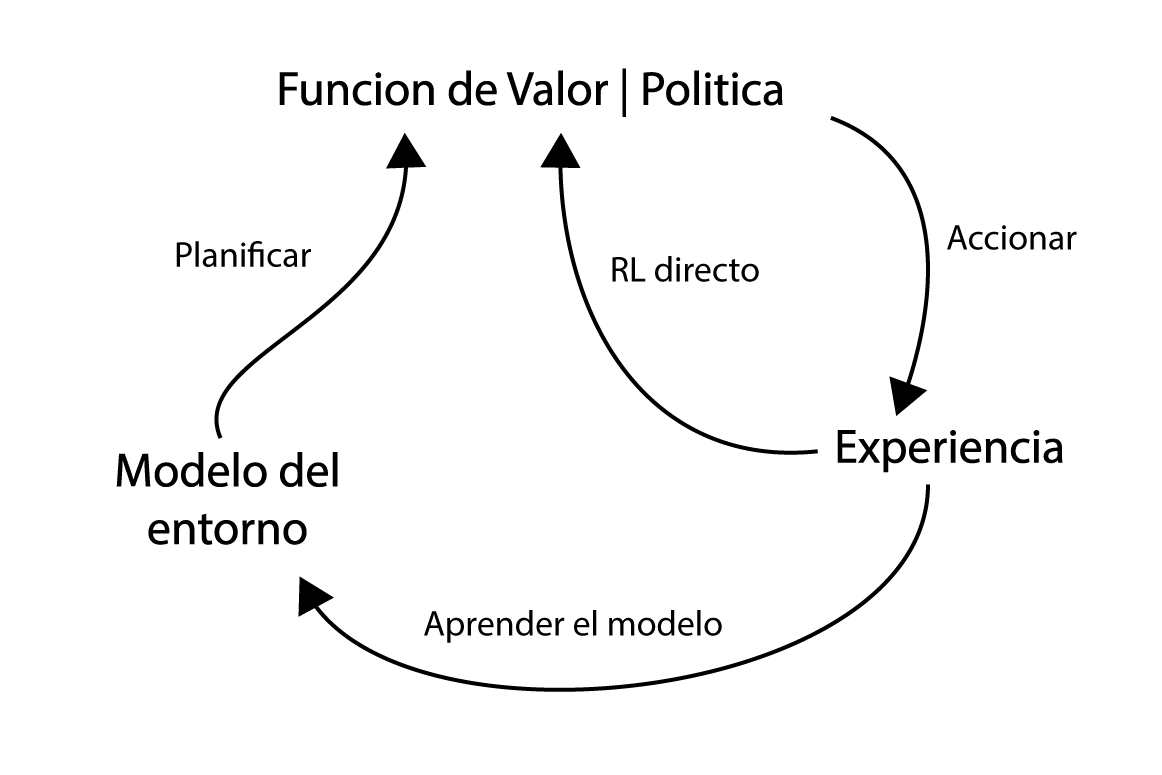
\includegraphics[width=0.7\textwidth]{Graphics/rl-strategies.png}
    \caption{Relaciones entre el aprendizaje, la planificación y la actuación.}
    \label{fig:rl-strategies}
\end{figure}

Dentro de los algoritmos  \textit{libres de modelo} existe otra caracterización basada en si se construye explícitamente o no la política del agente:

\begin{itemize}
\item En los métodos \textit{basados en políticas} se construye explícitamente una representación de una política y se mantiene en memoria durante el aprendizaje. Se puede citar los algoritmos de \textit{Policy Gradient}, \textit{Monte Carlos Tree Search}, \textit{Proximal Policy Optimization} (PPO) (\cite{schulman2017proximal})  entre otros.

\item En los métodos \textit{basados en valores} no se almacena ninguna política explícita, sólo una función de valor. La política es aquí implícita y puede derivarse directamente de la función de valor (elegir la acción con el mejor valor). Se puede citar los algoritmos de \textit{Q-Learning}, \textit{Deep Q-Learning}, \textit{SARSA}, entre otros.

\item Los algoritmos de \textit{Actor-crítico} tienen una mezcla de los dos anteriores. Se pueden citar algoritmos como \textit{AlphaZero} o \textit{Soft Actor-Critic} (SAC) (\cite{haarnoja2018soft}).
\end{itemize}

Los métodos on-policy intentan evaluar o mejorar la política que se utiliza para tomar las decisiones, mientras que los métodos off-policy evalúan o mejoran una política diferente a la utilizada para generar los datos. En el primer caso, el agente aprende la función de valor de la política que sigue en ese momento, mientras que en el segundo caso aprende la función de valor de la política que considera mejor en ese momento. Estas dos políticas suelen ser diferentes debido a la necesidad de explorar.

\subsection{Aprendizaje profundo por reforzamiento}

El aprendizaje profundo por refuerzo (Deep RL) es un subcampo del aprendizaje automático que combina el aprendizaje por refuerzo (RL) y el aprendizaje profundo. Incorpora el aprendizaje profundo a la solución, lo que permite a los agentes tomar decisiones a partir de datos de entrada no estructurados sin necesidad de ingeniería manual del espacio de estados. Los algoritmos de RL profunda son capaces de tomar datos de entrada muy grandes (por ejemplo, cada píxel representado en la pantalla de un videojuego) y decidir qué acciones realizar para optimizar un objetivo (por ejemplo, maximizar la puntuación del juego). (\cite{franccois2018introduction})

La mayoría de los experimentos que probaron las pruebas descritas en (\ref{section:state-of-the-art:evaluation-enviroments-for-generalization-on-rl-algoritms}) tanto como los usados en las experimentaciones de la solución que se presentará son de este tipo de algoritmos.

\section{Generalizacion en machine learning}\label{section:state-of-the-art:generalization-on-machine-learning}

La generalización es la capacidad de manejar situaciones (o tareas) que difieren de las situaciones anteriores. La inteligencia artificial se caracteriza como el rendimiento de un modelo en entradas que no formaban parte de sus datos de entrenamiento.

La capacidad generalización se basa fundamentalmente en las nociones relacionadas a la novedad e incertidumbre. Un sistema sólo puede generalizar ante información nueva que no pueda ser conocida de antemano ni por el sistema o por su creador. Dicha capacidad se pone en evidencia a medida que aumenta el dominio de las tareas y problemas que se pueden manejar (\cite{chollet2019measure}).

\subsection{Tipos de Generalizacion}\label{section:state-of-the-art:generalization-on-machine-learning:type-of-generalizations}

\begin{itemize}
\item \textit{Generalización centrada en el sistema:} es la capacidad de un sistema de aprendizaje para manejar situaciones que no ha encontrado antes. La noción formal de error de generalización en la teoría del aprendizaje estadístico pertenece aquí.

\item \textit{Generalización consciente del desarrollador:} es la capacidad de un sistema, ya sea de aprendizaje o estático, para manejar situaciones que ni el sistema ni el desarrollador del sistema han encontrado antes.
\end{itemize}

\subsection{Grados de Generalizacion}

Aunque los límites entre los grados de la escala de generalización son mayormente difusos y continuos, se ha agrupado en 4 niveles fundamentales de interés para el estudio (\cite{chollet2019measure}):

\begin{itemize}
\item \textit{Ausencia de generalización:} Sistemas en los que no hay incertidumbre no se muestra generalización. Por ejemplo, no se puede decir que un programa que juega a 4 en Línea mediante una iteración exhaustiva generalice a todas las configuraciones del tablero.

\item \textit{Generalización local o robustez:} Es la capacidad de un sistema para manejar nuevos puntos de una distribución conocida para una sola tarea o un conjunto bien delimitado de tareas conocidas, dado un muestreo suficientemente denso de ejemplos de la distribución (por ejemplo, la tolerancia a las perturbaciones previstas dentro de un contexto fijo). Por ejemplo, se puede decir que un clasificador de imágenes que puede distinguir imágenes RGB de 150x150 no vistas anteriormente que contienen gatos de las que contienen perros, después de haber sido entrenado con muchas de esas imágenes etiquetadas, realiza una generalización local. 

\item \textit{Generalización amplia o flexibilidad:} Es la capacidad de un sistema para manejar una amplia categoría de tareas y entornos sin más intervención humana. Esto incluye la capacidad de manejar situaciones que no podrían haber sido previstas por los creadores del sistema. Podría considerarse que refleja la capacidad del ser humano en un único y amplio ámbito de actividad (por ejemplo, las tareas domésticas o la conducción en el mundo real).

\item \textit{Generalización extrema:} Describe los sistemas abiertos con la capacidad de abordar tareas completamente nuevas que sólo comparten puntos comunes abstractos con situaciones previamente encontradas, aplicables a cualquier tarea y dominio dentro de un amplio alcance. Esto podría caracterizarse como adaptación a incógnitas desconocidas en una gama desconocida de tareas y dominios. Las formas biológicas de inteligencia (los humanos y posiblemente otras especies inteligentes) son el único ejemplo de un sistema de este tipo en este momento.
\end{itemize}

A esta lista se podría, en teoría, añadir una entrada más: \textit{La universalidad}, que extendería la generalidad más allá del ámbito de las tareas relevantes para los humanos, a cualquier tarea que pueda ser abordada de forma práctica dentro de nuestro universo (nótese que esto es diferente de cualquier tarea en absoluto, tal y como se entiende en los supuestos del teorema \textit{No Free Lunch} (\cite{wolpert1997no})).

Es importante destacar que el espectro de la generalización descrito anteriormente parece reflejar la organización de las capacidades cognitivas de los seres humanos tal y como se establece en las teorías de la estructura de la inteligencia en la psicología cognitiva donde se define el \textit{factor g} como una razón global y presente en el nivel de inteligencia del hombre. 
iv

\begin{figure}[ht!]
    \centering
    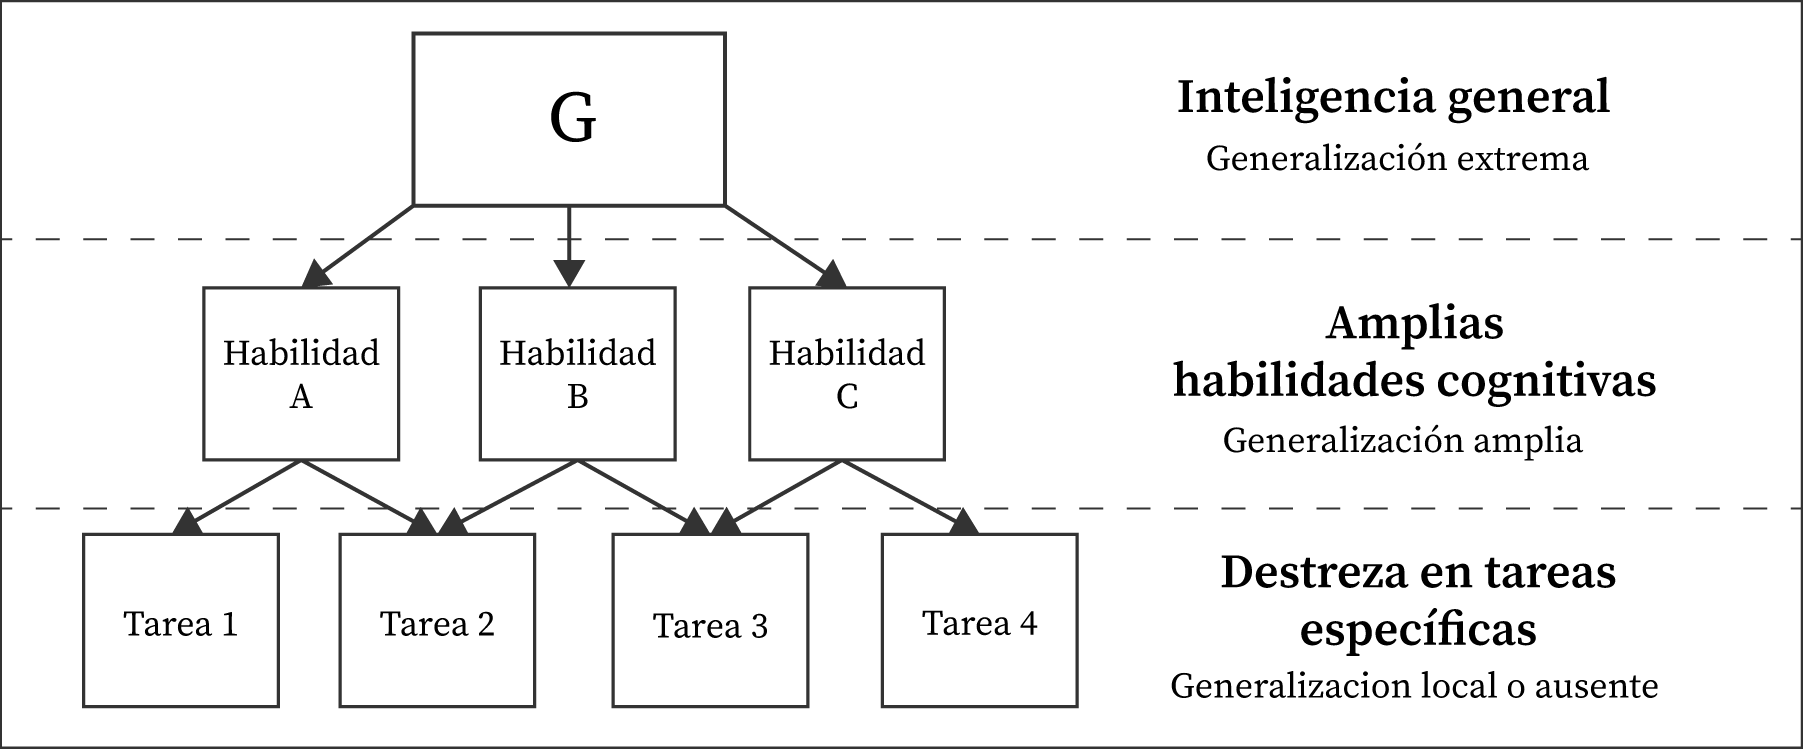
\includegraphics[width=0.7\textwidth]{Graphics/g-factor.png}
    \caption{Modelo jerárquico de las capacidades cognitivas y su correspondencia con el espectro de la generalización.}
    \label{fig:g-factor}
\end{figure}

\section{Métodos para la evaluación de algoritmos de aprendizaje automático}\label{section:state-of-the-art:evaluating-algoritms}

Las medidas de rendimiento que cuantifican la habilidad de un sistema en una tarea determinada han impulsado el éxito de la inteligencia artificial. No existe una forma única y formalizada de realizar una evaluación basada en la destreza. Entre los enfoques que han tenido éxito históricamente se encuentran:

\begin{itemize}
\item Revisión humana: Hacer que jueces humanos observen la respuesta de entrada-salida del sistema y la puntúan. Esta es la idea que subyace al Test de Turing (\cite{pinar2000turing}) y sus variantes. Este modo de evaluación rara vez se utiliza en la práctica, debido a que es caro, imposible de automatizar y subjetivo. Algunos sistemas de IA orientados al ser humano (en particular los chatbots comerciales) lo utilizan como uno de los múltiples mecanismos de evaluación.

\item Análisis en Caja-Blanca (White-Box Analysis): Inspeccionar la implementación del sistema para determinar su respuesta de entrada-salida y puntuarla. Esto es más relevante para los algoritmos que resuelven una tarea totalmente descrita en un entorno totalmente descrito en el que todas las entradas posibles pueden enumerarse explícitamente o describirse analíticamente y a menudo tomaría la forma de una prueba de optimalidad.

\item Por Confrontación (Peer Confrontation): Hacer que el sistema compita contra otras IAs o contra humanos. Este es el modo de evaluación preferido para los juegos de jugador contra jugador, como el ajedrez.

\item Comparaciones de referencia (Benchmarks): Hacer que el sistema produzca resultados para un conjunto de pruebas de entradas (o entornos) para los que se conoce el resultado deseado, y puntuar la respuesta.
\end{itemize}

Los \textit{Benchmarks}, en particular, han sido un importante motor de progreso en la IA, porque son reproducibles (el conjunto de pruebas es fijo), justos (el conjunto de pruebas es el mismo para todos), escalables (es barato realizar la evaluación muchas veces), fáciles de configurar y lo suficientemente flexibles como para ser aplicables a una amplia gama de tareas posibles. Los puntos de referencia han sido a menudo más impactantes en el contexto de una competición entre diferentes equipos de investigación.

La robustez de los sistemas que se desarrollan, en particular los modelos de Deep Learning, suele ser problemática. Esto se debe en gran parte al hecho de que la mayoría de los benchmarks no prestan mucha atención a la evaluación formal de la robustez y a la cuantificación de la generalización, y por lo tanto pueden ser resueltos a través de atajos que el descenso de gradiente es apto para explotar. La generalización entre tareas sigue siendo difícil para los algoritmos de aprendizaje profundo por refuerzo más avanzados. Aunque los agentes entrenados pueden resolver tareas complejas, les cuesta transferir su experiencia a nuevos entornos. Los agentes que dominan diez niveles de un videojuego suelen fracasar estrepitosamente cuando se enfrentan por primera vez al undécimo. Los humanos pueden generalizar sin problemas en tareas similares, pero esta capacidad está ausente en los agentes de la realidad virtual. Los agentes se especializan demasiado en los entornos encontrados durante el entrenamiento (\cite{cobbe2019quantifying}). A este fenómeno se le denomina sobre \textit{overfitting}. Se reconoce ampliamente que los agentes de RL son propensos a la sobre adaptación (\cite{zhang2018study}), pero los puntos de referencia de RL más comunes siguen fomentando el entrenamiento y la evaluación en el mismo conjunto de entornos. (\cite{nichol2018gotta}) 

\section{Una buena evaluación de Inteligencia}\label{section:state-of-the-art:a-good-measure-of-inteligence}

\subsection{¿Qué es la Inteligencia?}
Existen muchas definiciones posibles de inteligencia, varían según el campo de estudio y pueden ser válidas en muchos contextos diferentes. En este documento la definición que nos es útil y medible se puede definir de la siguiente manera:

\begin{quote}
   \textit{ La inteligencia de un sistema es una medida de su eficiencia en la adquisición de habilidades sobre un ámbito de tareas, con respecto a los antecedentes, la experiencia y la dificultad de generalización.}
\end{quote}

Esta definición de inteligencia engloba el meta-aprendizaje de los conocimientos previos, la memoria y la inteligencia fluida. Es distinta de la destreza en sí misma: la destreza no es más que el resultado del proceso de la inteligencia. El propósito de esta definición es ser procesable, servir como un cambio de perspectiva útil para la investigación de amplias capacidades cognitivas, y funcionar como una base cuantitativa para nuevos puntos de referencia de inteligencia general (\cite{chollet2019measure}).

\subsection{Inteligencia en la perspectiva antropocéntrica}

Un punto central de este documento es que la inteligencia general no es una propiedad binaria que un sistema posee o carece. Se trata de un espectro, ligado a: un ámbito de aplicación, que puede ser más o menos amplio, el grado de eficacia con el que el sistema traduce sus conocimientos previos y su experiencia en nuevas habilidades en el ámbito considerado, y por último al grado de dificultad de generalización que representan los distintos puntos del ámbito considerado. Además, el valor de un ámbito de aplicación sobre otro es totalmente subjetivo; no nos interesa (ni se persive como inteligente) un sistema cuyo ámbito de aplicación no tuviera ninguna intersección con el nuestro. (\cite{chollet2019measure})

La investigación sobre el desarrollo de la amplitud de los sistemas de IA (hasta llegar a la IA genérica, es decir, la IA con un grado de generalidad comparable al de la inteligencia humana) se centra en definir, medir y desarrollar una forma de inteligencia específicamente similar a la humana (\cite{goertzel2012architecture}), y que se compare el progreso específicamente con la inteligencia humana (altamente especializada). Esto no se debe a que la inteligencia que difiere en gran medida de la nuestra no pueda existir o no tenga valor; más bien, se reconoce que la caracterización y la medición de la inteligencia es un proceso que debe estar vinculado a un ámbito de aplicación bien definido, y en este momento, el espacio de las tareas relevantes para el ser humano es el único ámbito que se puede abordar y evaluar de forma significativa. Por lo tanto, al contrario de otras perspectivas, como la Psicometría Universal (\cite{hernandez2014universal}) o la Inteligencia Universal (\cite{legg2007universal}), que rechazan por completo el antropocentrismo y pretenden medir toda la inteligencia con una única escala absoluta. Un marco de referencia antropocéntrico no sólo es legítimo, sino necesario. (\cite{chollet2019measure})

La comparación entre dos sistemas inteligentes debe ser justa, teniendo en cuenta los prejuicios y experiencias que ambos poseen. Por esto se hace necesario separar los elementos del conocimiento de forma tal que puedan ser comparables. En el caso de los humanos una forma particular de verlo sería la siguiente:

\begin{itemize}
    \item \textbf{Prejuicios de bajo nivel}: Conocimientos sobre nuestro propio espacio sensoriomotor. Reflejos e instintos innatos.
    \item \textbf{Prejuicios de metaaprendizaje}: Rigen nuestras estrategias de aprendizaje y capacidades de adquisición de conocimientos. Es la inteligencia en sí misma. La forma en que se transforma experiencias en conocimientos y habilidades.
    \item \textbf{Conocimientos previos de alto nivel}: Conocimientos sobre los objetos y fenómenos de nuestro entorno externo.
\end{itemize}

Estos prejuicios no son una limitación a nuestra capacidad de generalización; al contrario, son su fuente, la razón por la que los humanos son capaces de adquirir ciertas categorías de habilidades con una eficiencia notable. El mensaje central del teorema No Free Lunch (\cite{wolpert1997no}) es que para aprender de los datos hay que hacer suposiciones sobre ellos: la naturaleza y la estructura de las suposiciones innatas que hace la mente humana son precisamente las que le confieren sus poderosas capacidades de aprendizaje. 

\subsection{¿Cuál es la lista exacta de conocimientos previos con los que nacen los humanos?}\label{section:state-of-the-art:a-good-measure-of-inteligence:human-prios}

El Conocimiento Básico identifica cuatro amplias categorías de supuestos innatos que forman los cimientos de la cognición humana  (\cite{spelke2007core}), y que son compartidos en gran medida por los parientes no humanos.

\begin{itemize}

\item Objetualidad y física elemental: El ser humano supone que su entorno debe dividirse en objetos caracterizados por los principios de cohesión (los objetos se mueven como conjuntos continuos, conectados y delimitados), persistencia (los objetos no dejan de existir repentinamente y no se materializan de repente) y contacto (los objetos no actúan a distancia y no pueden interpenetrarse).

\item Agilidad y dirección de objetivos: Los seres humanos suponen que, mientras que algunos objetos de su entorno son inanimados, otros son agentes, que poseen intenciones propias, que actúan para alcanzar objetivos (por ejemplo, si se ve que un objeto A sigue a otro objeto B en movimiento, se puede deducir que A persigue a B y que B huye de A), y que muestran eficacia en sus acciones dirigidas a objetivos. Se espera que estos agentes actúen de forma contingente y recíproca.

\item Números naturales y aritmética elemental: Los seres humanos poseen representaciones numéricas innatas y abstractas para los números pequeños, que pueden aplicarse a entidades observadas a través de cualquier modalidad sensorial. Estas representaciones numéricas pueden sumarse o restarse, y pueden compararse entre sí u ordenarse.

\item Geometría y topología elementales: Este sistema de conocimiento básico recoge las nociones de distancia, orientación y relaciones de entrada y salida de los objetos de nuestro entorno y de nosotros mismos. Es la base de la facilidad innata de los seres humanos para orientarse con respecto a su entorno y navegar por entornos 2D y 3D.
\end{itemize}

\subsection{Características de una buena evaluación de inteligencia en esta perspectiva}

Para lograr un proceso de evaluación justo es necesario definir, tomando lo planteado en las secciones anteriores, las características que cumpla todo entorno de evaluación de inteligencia con capacidades de generalización extremas:

\begin{itemize}
\item Ámbito de la Evaluación explícito: Las tareas deben ser realizables de forma similar. Respetando las destrezas que se puedan expresar.
\item Replicabilidad y Reproducibilidad: Debe poder ser reproducido por otros investigadores. En caso de utilizar los mismo parámetros, arrojar resultados similares.  
\item Valorar la generalización por encima de la destreza: No debe limitarse a medir el desempeño en una tarea, sino a la evaluación de la adquisición de nuevas habilidades y el uso de estas para resolver nuevas tareas.
\item Medir la generalización consciente del desarrollador: Debe contener tareas no conocidas por los desarrolladores.
\item Eficiencia de muestras: Controlar la cantidad de experiencia que se brinda para que sean manifiestas las habilidades cognitivas abstractas.
\item Prejuicios de conocimientos explícitos: Definir el conjunto de premisas de Conocimiento previo de forma explícita y acorde a los fundamentos antropocéntricos planteados.
\item Evaluación de humanos y máquinas: Debe funcionar para humanos y máquinas para crear un punto de comparación válido.
\item Tareas fundamentalmente diferentes: Debe justificar la dificultad de generalización entre las pruebas.
\end{itemize}

\section{Entornos de evaluación de Inteligencia}\label{section:state-of-the-art:inteligence-evaluation-enviroments}

\subsection{Juego de Imitación}

El juego original descrito por Turing es una prueba de la capacidad de una máquina para mostrar un comportamiento inteligente equivalente o indistinguible del de un ser humano. Proponía un juego que involucra tres participantes: el jugador A es un hombre, el jugador B es una mujer y el interrogador. En el juego, el interrogador no tiene contacto visual con ninguno de los otros jugadores y se puede comunicar con ellos por medio de notas escritas. Al hacerles preguntas, el interrogador intenta determinar cuál de los dos es el hombre y cuál la mujer. El jugador A intentará engañar al interrogador haciéndole escoger erróneamente mientras que el jugador B le auxiliará al interrogador en escoger al jugador correcto. 

Turing propuso que el rol del jugador A lo cumpliera una computadora para que esta tuviera que pretender ser mujer e intenta guiar al interrogador a la respuesta incorrecta. El éxito de la computadora sería determinado al comparar el resultado del juego cuando el jugador A es la computadora junto con el resultado del juego cuando el jugador A es un hombre. Turing afirmó que si el interrogador decide erróneamente tan frecuentemente cuando el juego es jugado con la computadora, como cuando el juego es jugado entre un hombre y una mujer, se podría argumentar que la computadora es inteligente. (\cite{pinar2000turing})

\subsection{Prueba del Café}

Consiste en que la máquina demuestre la capacidad de poder acceder una cocina al azar y preparar una taza de café. De este modo, la máquina debe ser capaz de localizar la cafetera, encontrar el café, poner agua, encontrar una taza, y toda una serie de pequeñas operaciones que para un ser humano resultan incluso intuitivas, pero que para una máquina requieren una gran cantidad de cálculos.

La prueba fue desarrollada por Wozniak, un investigador pionero en el estudio de la inteligencia artificial general, y pone en evidencia la llamada paradoja de Moravec (\cite{rotenberg2013moravec}): algunas tareas que son difíciles para los seres humanos (como multiplicar cifras muy altas) no entrañan ninguna dificultad para una máquina, pero otras acciones muy simples, incluso realizables por un niño, como doblar la ropa, requieren grandes cantidades de cálculos.

Existen otras pruebas propuestas por Goertzel, en una de ellas un estudiante universitario robot se debe matricular en una universidad, tomar y aprobar las mismas clases que los humanos y obtener un título.

\subsection{The bica cognitive decathlon}

BICA (Biologically-Inspired Cognitive Architectures) (\cite{mueller2007bica}) tiene como objetivo la generación de modelos de arquitectura cognitiva basados en principios de la psicología y la neurociencia. 

Este proyecto está motivado por la creencia de que la investigación tradicional sobre inteligencia artificial se ha topado con un muro en su intento de desarrollar agentes verdaderamente inteligentes. Aunque los agentes pueden ser diseñados para realizar tareas específicas de forma excelente, suelen ser bastante frágiles, incapaces de enfrentarse a situaciones imprevistas y de aprender de otros. 

Un conjunto de pruebas ha sido diseñado para evaluar el rendimiento de dichos agentes en una variedad de situaciones que cubren algunas habilidades básicas cognitivas, perceptivas y motoras, típicas de un niño humano de dos años. Estas incluyen tareas de comportamiento relacionadas con la búsqueda, la navegación, la manipulación, la memoria, el lenguaje y tres vías de conocimiento procedimental: instrucción, demostración y exploración.

Las pruebas tienen tres componentes distintos: un total de cuatro escenarios de retos integradores que apoyan los objetivos de construcción de agentes cognitivos coherentes, sistemáticos e integrados; un conjunto de tareas enfocadas que pueden determinar mejor hasta qué punto las competencias cognitivas básicas coincide con las capacidades de los humanos; y evaluaciones de bio-validez para determinar hasta qué punto la arquitectura de los agentes se asemeja al cerebro humano.
 
Estos exámenes de tres niveles se diseñaron para comprobar si los sistemas son flexibles, completos y capaces de realizar tareas en situaciones complejas, sin dejar de hacerlas de forma similar a los humanos.

\subsection{Olimpiadas de Turing}

Un grupo de expertos en inteligencia artificial se reunieron para discutir cómo avanzar más allá del test de Turing, en el marco de la conferencia AAAI de inteligencia artificial en Austin, Texas. Asumieron la tarea de elaborar un \textit{campeonato de Turing} con un nuevo conjunto de desafíos que ayuden a desarrollar la investigación de AI. La idea de este grupo de trabajo es desarrollar una serie de desafíos que puedan evaluar diferentes tipos de inteligencia.

\begin{itemize}
    \item Test de Ikea: Un robot que sea capaz de armar muebles tan solo leyendo las instrucciones, debe ser capaz de ver las partes, interpretar las instrucciones y eventualmente tener las habilidades motoras para unirlas, guiado por un programa de AI. Esto tiene varias etapas y podría comenzar con simulaciones antes de empezar con robots reales.

    \item El esquema de Winograd: Una prueba basada en el lenguaje que requiere algo como el sentido común de los humanos. Fue propuesto por el científico computacional Hector Levesque en 2011. Los esquemas de Winograd les dan una frase a los participantes, luego formulan una simple pregunta sobre esa frase. Son preguntas muy fáciles para los humanos, pero requieren una comprensión del lenguaje relativamente profunda. Descritas como frases que no puedes entender a menos que entiendas el mundo.
    
    \item Una tercera prueba fue sugerida por Gary Marcus, un profesor de psicología en NYU, propuso pedirle a un computador que viera un video que no haya visto antes y hacerle preguntas sobre él. Preguntas al estilo: ¿Por qué Rusia invadió Crimea? o ¿Por qué Walter White quiso matar a Jessie? Es decir, crear un evento donde una máquina pueda responder preguntas periodísticas sobre imágenes, video y audio.

    \item Otras ideas que salieron del encuentro fue desafiar a una AI a jugar un nuevo videojuego como si fuera un niño de 12 años, o decirle a un profesor digital que aprenda un nuevo tópico y lo enseñe igual (o mejor) que un humano.
\end{itemize}

\section{Entornos de evaluación de la capacidad de generalización en algoritmos RL}\label{section:state-of-the-art:evaluation-enviroments-for-generalization-on-rl-algoritms}

\subsection{The Arcade Learning Environment}\label{section:state-of-the-art:evaluation-enviroments-for-generalization-on-rl-algoritms:ALE}

ALE está construido sobre Stella 1, un emulador de Atari 2600 de código abierto. Permite al usuario interactuar con la Atari 2600 recibiendo los movimientos del joystick, enviando información de la pantalla y/o de la RAM, y emulando la plataforma. ALE también proporciona una capa de manejo de juegos que transforma cada juego en un problema estándar de aprendizaje por refuerzo, identificando la puntuación acumulada y si el juego ha terminado. Por defecto, cada observación consiste en una única pantalla de juego (frame): una matriz 2D de píxeles de 7 bits, de 160 píxeles de ancho por 210 de alto. El espacio de acción está formado por las 18 acciones discretas definidas por el mando del joystick. La capa de gestión del juego también especifica el conjunto mínimo de acciones necesarias para jugar a un determinado juego, aunque ninguno de los resultados de este artículo hace uso de esta información. Cuando se ejecuta en tiempo real, el simulador genera 60 fotogramas por segundo, y a toda velocidad emula hasta 6000 fotogramas por segundo. La recompensa en cada paso de tiempo se define juego por juego, normalmente tomando la diferencia de puntuación o puntos entre fotogramas. Un episodio comienza en el primer fotograma después de que se emita un comando de reinicio, y termina cuando el juego termina. La capa de gestión del juego también ofrece la posibilidad de terminar el episodio después de un número predefinido de fotogramas. Por lo tanto, el usuario tiene acceso a varias docenas de juegos a través de una única interfaz común, y añadir soporte para nuevos juegos es relativamente sencillo. (\cite{bellemare2013arcade})

\begin{figure}[ht!]
    \centering
    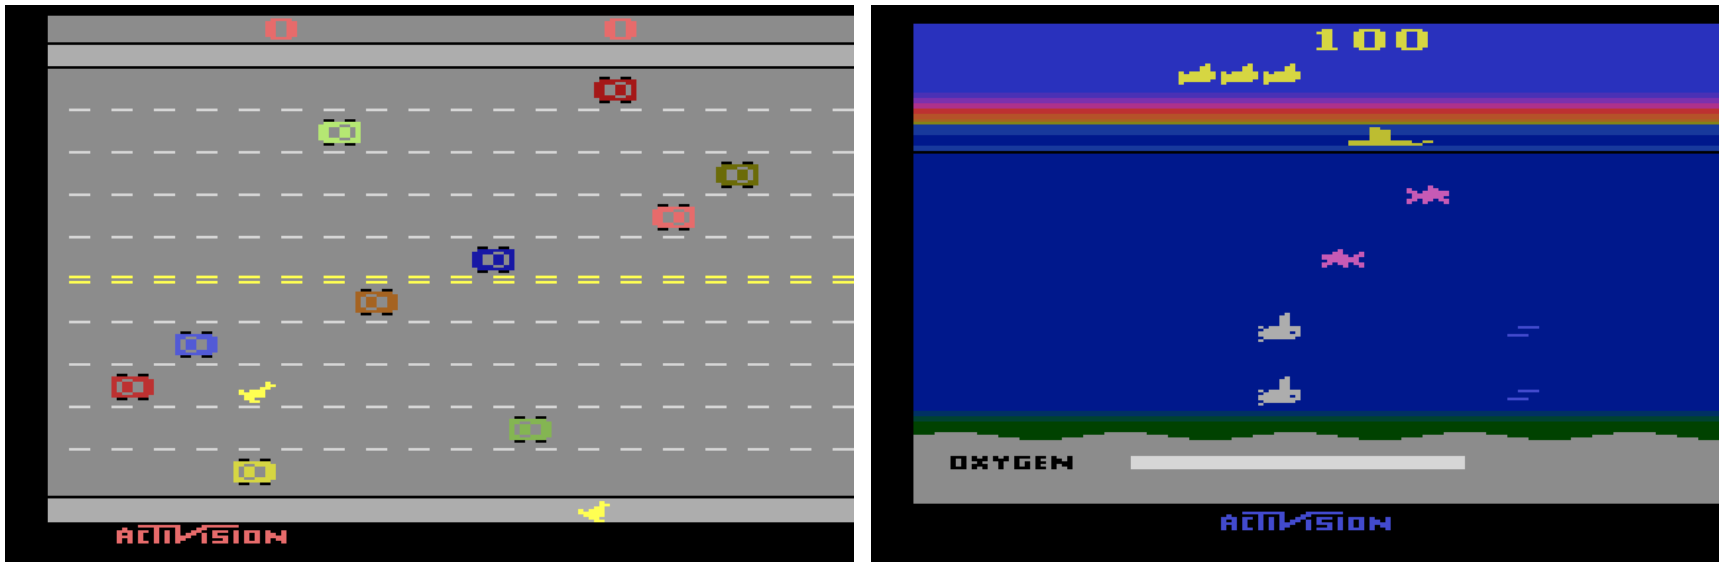
\includegraphics[width=0.7\textwidth]{Graphics/ale.png}
    \caption{Capturas de pantalla de varios juegos de ALE}
    \label{fig:ale}
\end{figure}

En (\cite{farebrother2018generalization}) también se aborda este problema, reconociendo activamente que la confusión de los entornos de entrenamiento y prueba ha contribuido a la falta de regularización en la RL profunda. Proponen utilizar diferentes modos de juego de Atari 2600 para medir la generalización. Recurren al aprendizaje supervisado en busca de inspiración, descubriendo que tanto la regularización L2 (\cite{krogh1991simple}) como el abandono pueden ayudar a los agentes a aprender características más generales.

Desde el ajedrez (\cite{silver2017mastering}) hasta el Go (\cite{silver2016mastering}), desde los antiguos juegos de Atari (\cite{bellemare2013arcade}) hasta Starcraft 2 (\cite{vinyals2017starcraft}), se ve una gran variedad de entornos desafiantes en los que la IA supera ahora a los humanos. Éxitos como estos en el aprendizaje por refuerzo incluso han dado lugar a la transferencia de agentes entrenados al mundo real para manipulaciones robóticas (\cite{andrychowicz2020learning}). Estos impresionantes resultados son solo un primer paso hacia agentes que puedan interactuar de forma robusta con sus entornos. En estos entornos, la mayoría de las tareas utilizadas para el entrenamiento son idénticas, o extremadamente similares, a las utilizadas para las pruebas. Aunque el agente no siempre ha estado expuesto a las tareas de prueba durante el entrenamiento, probablemente ha estado expuesto a tareas extraídas de la misma distribución. Esto da lugar a agentes que alcanzan un rendimiento sobrehumano en problemas específicos, pero que son incapaces de generalizar (\cite{packer2018assessing}).

\subsection{CoinRun}

El entorno CoinRun tiene como propósito evaluar el rendimiento de la generalización de los agentes. El objetivo de cada nivel de CoinRun es sencillo: recoger la única moneda que se encuentra al final del nivel. El agente controla un personaje que aparece en el extremo izquierdo y la moneda aparece en el extremo derecho. Entre el agente y la moneda hay varios obstáculos, tanto fijos como no fijos. La colisión con un obstáculo provoca la muerte inmediata del agente. La única recompensa en el entorno se obtiene al recoger la moneda, y esta recompensa es una constante positiva fija. El nivel termina cuando el agente muere, se recoge la moneda o después de 1000 pasos de tiempo (\cite{cobbe2019quantifying}).

\begin{figure}[ht!]
    \begin{subfigure}
      \centering
      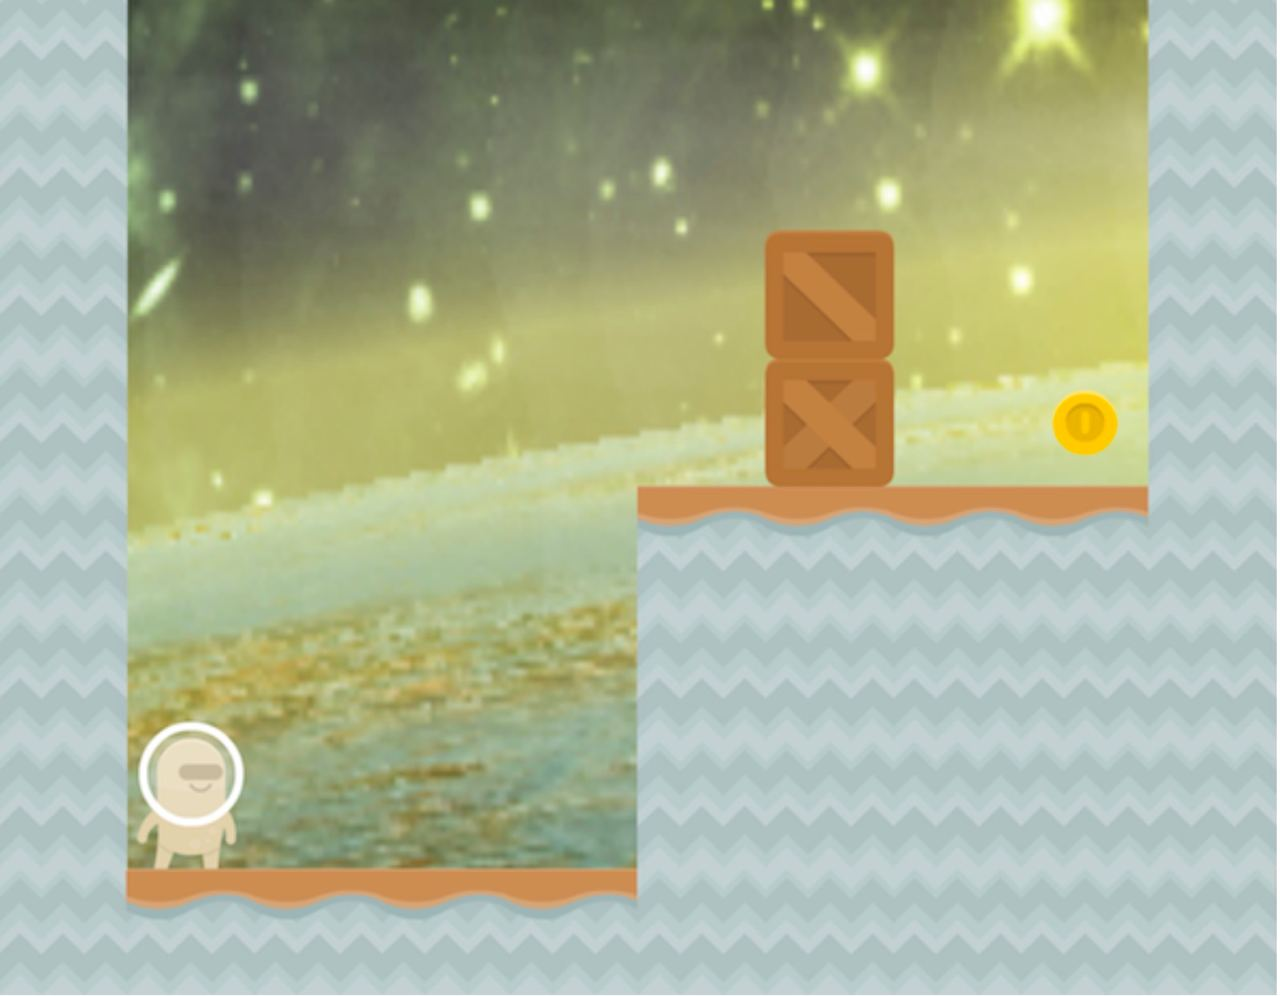
\includegraphics[width=0.4\textwidth]{Graphics/coinrun_1.jpeg}
      \label{fig:coinrun1}
    \end{subfigure}%
    \begin{subfigure}
      \centering
      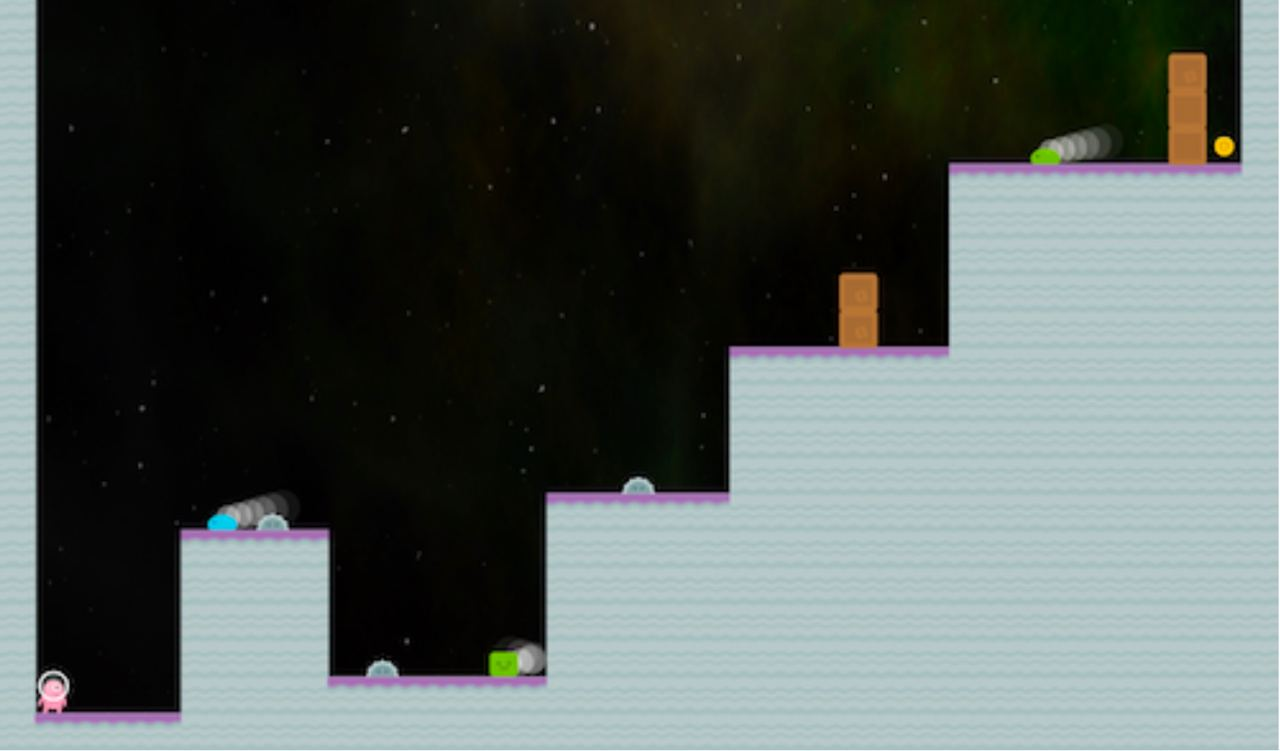
\includegraphics[width=0.4\textwidth]{Graphics/coinrun_2.jpeg}
      \label{fig:coinrun2}
    \end{subfigure}%
    \caption{Niveles de CoinRun con diferente dificultad}
    \label{fig:coinrun}
\end{figure}

El juego CoinRun esta diseñado para que sea manejable para los algoritmos existentes. Es decir, dado un número suficiente de niveles de entrenamiento y un tiempo de entrenamiento suficiente, los algoritmos probados aprenden una política casi óptima para todos los niveles de CoinRun. Cada nivel se genera de forma determinista a partir de una semilla dada, lo que proporciona a los agentes acceso a un suministro de datos de entrenamiento arbitrariamente grande y fácilmente cuantificable. CoinRun imita el estilo de juegos como Sonic (\cite{nichol2018gotta}), pero es mucho más sencillo. Para evaluar la generalización, esta simplicidad puede ser ventajosa. Los niveles varían mucho en dificultad, por lo que su distribución y organización forma naturalmente un plan de estudios para el agente (\cite{cobbe2019quantifying}).

CoinRun está diseñado para ser lo suficientemente simple como para que los niveles individuales sean fáciles de resolver cuando se entrena, pero la tarea es crear un agente que pueda resolver variaciones no vistas. La generación procedural de niveles y organización de dificultad tiene un efecto positivo en la evaluación de la generalización apoyada por la unión a las técnicas sugeridas para evitar sobreajuste en el entrenamiento. No define explícitamente las premisas de conocimiento que deberían poseer los agentes para ser evaluados y la simplicidad de las tareas impiden su uso como prueba para niveles de generalización más amplios.

\subsection{Procgen}

Procgen Benchmark consta de 16 entornos únicos diseñados por sus creadores e inspirados por (\cite{bellemare2013arcade}) para medir tanto la eficiencia de las muestras como la generalización en el aprendizaje por refuerzo. Estos entornos se benefician en gran medida del uso de la generación de contenido proceduralmente, la creación algorítmica de un suministro casi infinito de contenido altamente dominado. En estos entornos, emplear la generación procedural es mucho más eficaz que confiar en contenidos fijos diseñados por el ser humano. (\cite{cobbe2020leveraging})

La lógica de generación procedural rige el diseño de los niveles, la selección de los recursos del juego, la ubicación y los tiempos de aparición de las entidades, y otros detalles específicos del juego. Para dominar cualquiera de estos entornos, los agentes deben aprender una política que sea robusta en todos los ejes de variación (\cite{cobbe2020leveraging}). El aprendizaje de una política de este tipo es más desafiante y más relevante que el ajuste excesivo a un puñado de niveles fijos, como en el caso de ALE visto en \ref{section:state-of-the-art:evaluation-enviroments-for-generalization-on-rl-algoritms:ALE}. Estas cualidades de Procgen le permiten crear entornos para probar diferentes características de algoritmos de aprendizaje por reforzamiento, tales como la exploración, capacidad de memoria, y generalización local.

Para facilitar la ejecución Procgen presenta un espacio fijo de observaciones y acciones. Contando observaciones de tamaño $64*64*3(RGB)$ y $15$ acciones posibles, donde cada entorno define cuales de estas son aplicables. (\cite{cobbe2020leveraging})

Entre los de entornos similares se encuentran \textbf{OpenIA Gym} (\cite{brockman2016openai}), \textbf{Quake III Arena} (\cite{jaderberg2019human}) y \textbf{Obstacle Tower} (\cite{juliani2019obstacle}) el cual es un nuevo juego en 3D basado en la venganza de Moctezuma (Fig. \ref{fig:tower}), uno de los juegos Atari más difíciles (para la IA), cuyas fases se generan de forma procedural.

\begin{figure}[ht!]
    \centering
    \begin{subfigure}
      \centering
      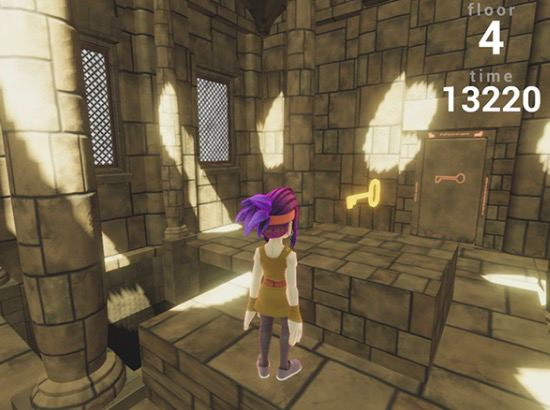
\includegraphics[width=0.4\textwidth]{Graphics/tower-1.jpeg}
      \label{fig:tower1}
    \end{subfigure}%
    \begin{subfigure}
      \centering
      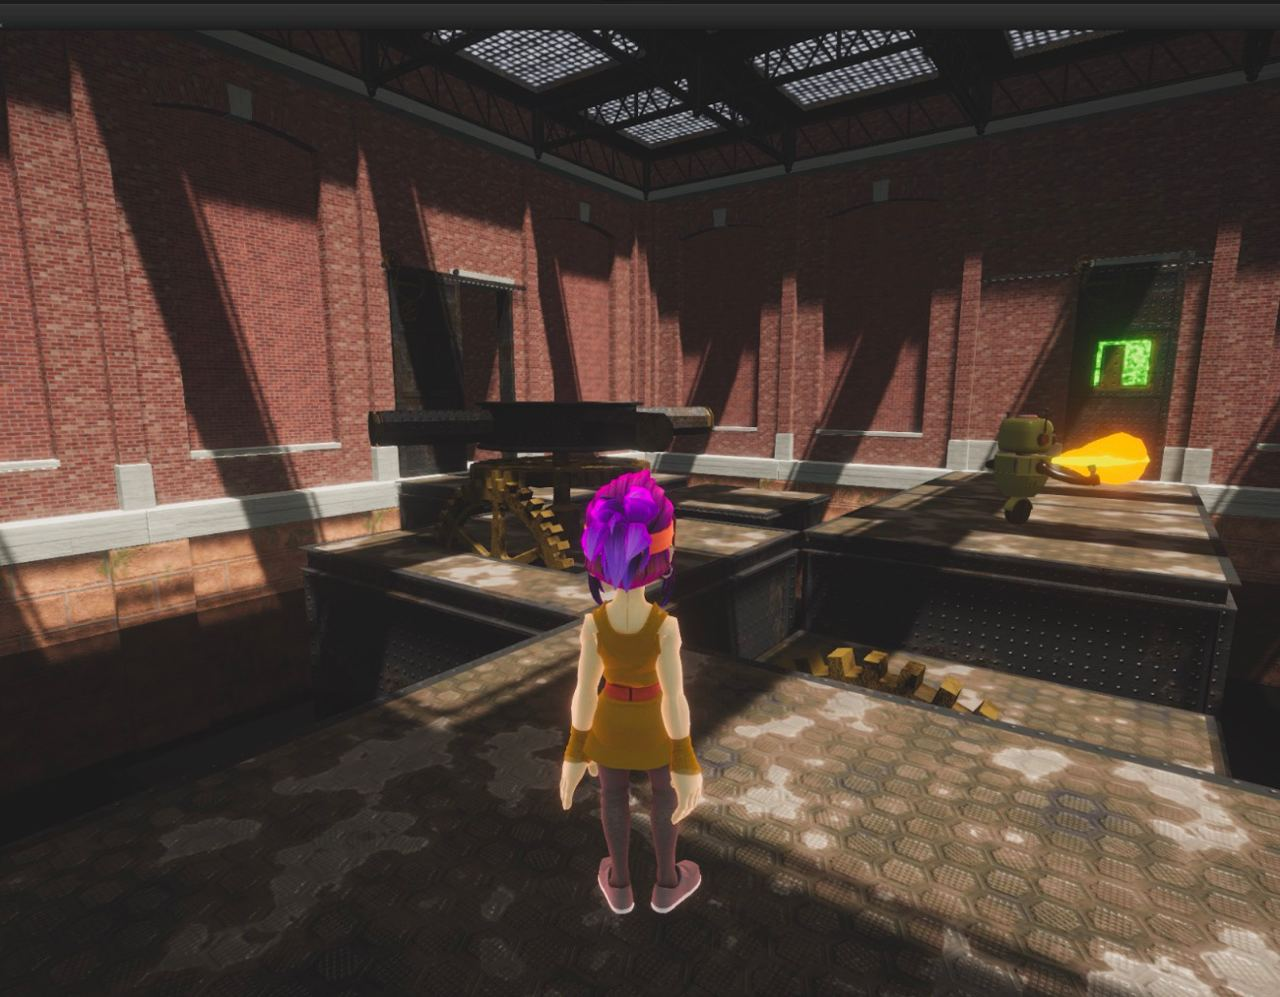
\includegraphics[width=0.4\textwidth]{Graphics/tower-2.jpeg}
      \label{fig:tower2}
    \end{subfigure}%
    \caption{Niveles de Obstacle Tower}
    \label{fig:tower}
\end{figure}

\begin{figure}[ht!]
    \centering
    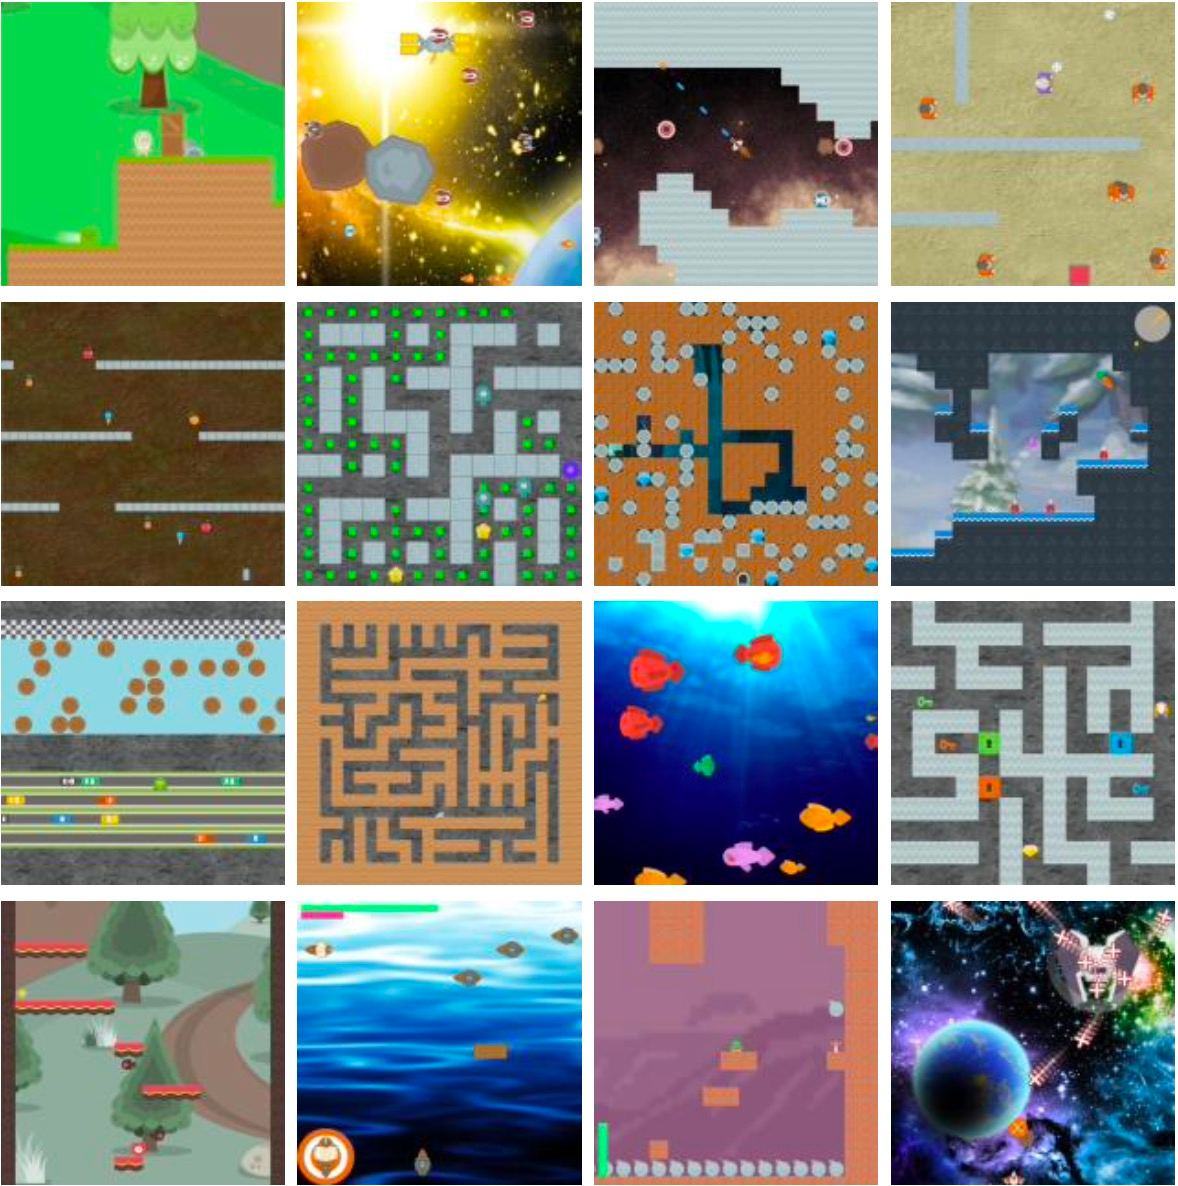
\includegraphics[width=0.7\textwidth]{Graphics/procgen.jpeg}
    \caption{Capturas de pantalla de varios juegos de Procgen}
    \label{fig:procgen}
\end{figure}

\subsection{The Animal-AI Environment}

El entorno Animal-AI es una nueva plataforma de experimentación y evaluación de IA que implementa la cognición. Está diseñado para contener sólo los ingredientes necesarios para realizar pruebas cognitivas construidas a partir de la percepción y la navegación. Comienza con tareas simples pero cruciales que muchos animales son capaces de resolver. Éstas incluyen la maximización de la recompensa, la física intuitiva, la permanencia de los objetos y el razonamiento causal simple. Al imitar las tareas y los protocolos de la cognición animal, se puede evaluar mejor el progreso de la IA de dominio general. (\cite{beyret2019animal})

\begin{figure}[ht!]
    \centering
    \begin{subfigure}
      \centering
      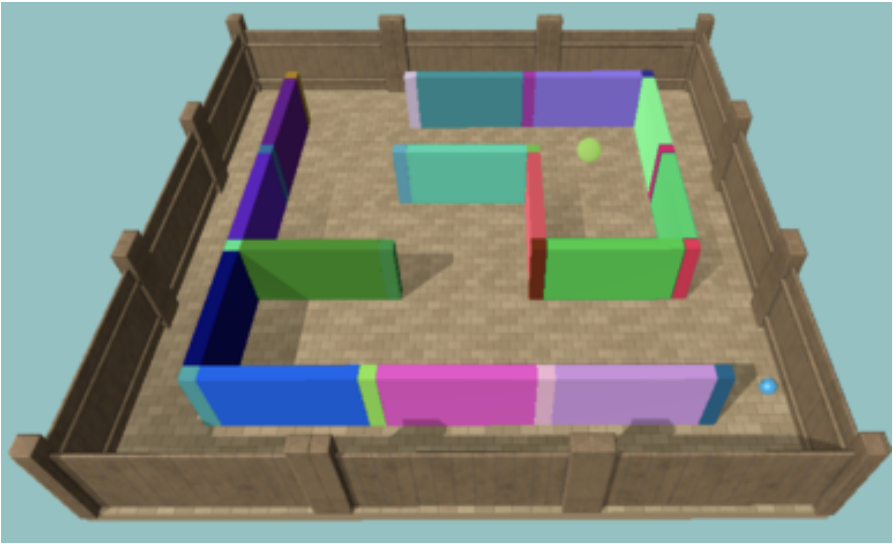
\includegraphics[width=0.4\textwidth]{Graphics/animal_1.png}
      \label{fig:animal1}
    \end{subfigure}%
    \begin{subfigure}
      \centering
      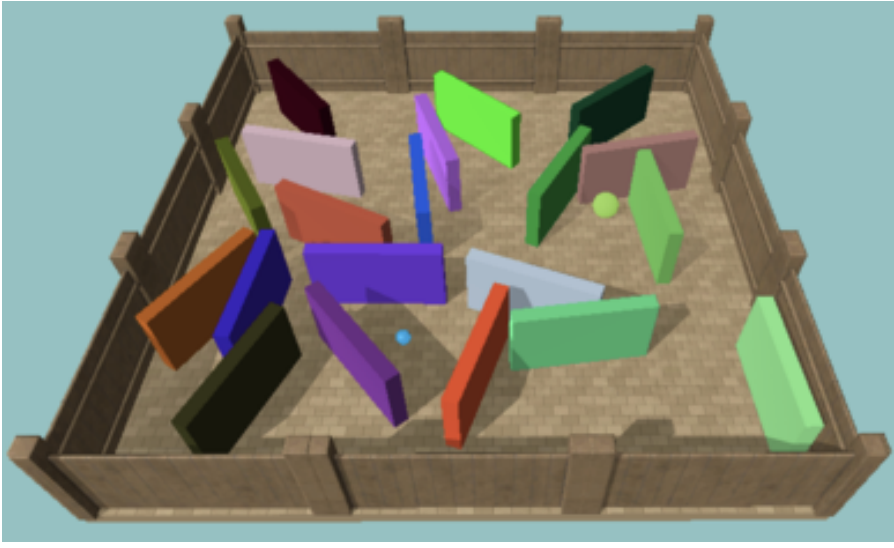
\includegraphics[width=0.4\textwidth]{Graphics/animal_3.png}
      \label{fig:animal2}
    \end{subfigure}%
    \caption{Niveles de Animal IA-Environment. A la izquierda X a la derecha Y.}
    \label{fig:animal}
\end{figure}

Inspirándose en la extensa literatura sobre la cognición animal, Animal-IA presenta un entorno que mantiene todos los elementos positivos de los entornos de juego estándar, pero que está diseñado explícitamente para probar la cognición artificial de tipo animal. Los experimentos son comparables entre el entorno de Animal-AI y la literatura sobre cognición animal, ya que imita la forma en que un experimentador construiría un entorno de pruebas para un animal. El entorno posee un API en python para su interacción y utiliza Unity ML (\cite{juliani2018unity}) para la simulación de las pruebas.

La batería de pruebas de Animal-AI se lanzó como parte de una competición junto con el entorno de Animal- AI. El formato de la competición permite evaluar el rendimiento en tareas totalmente ocultas.

\subsection{Project Malmo, un meta-entorno de pruebas en Minecraft}\label{section:state-of-the-art:evaluation-enviroments-for-generalization-on-rl-algoritms:malmo}

\begin{figure}[ht!]
    \centering
    \begin{subfigure}
      \centering
      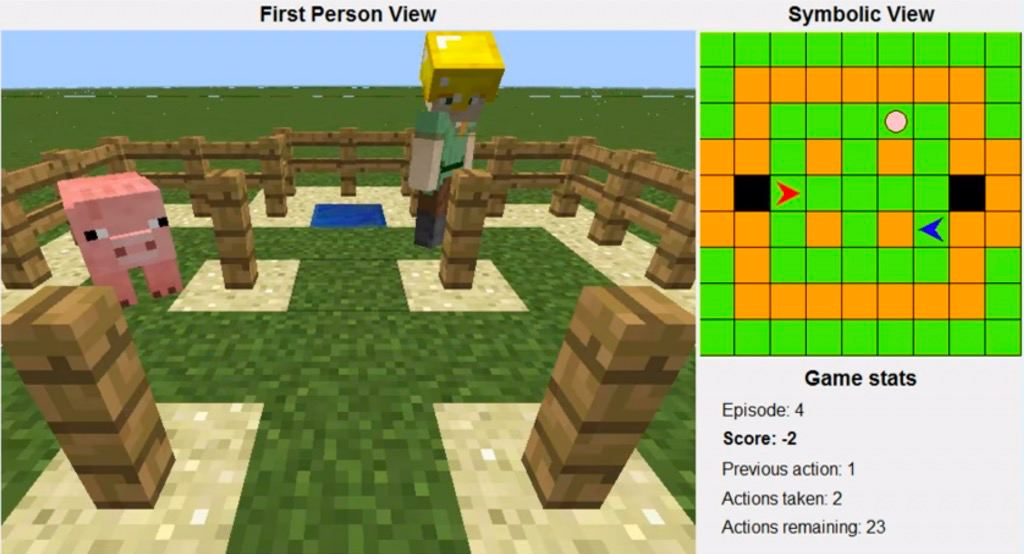
\includegraphics[width=0.4\textwidth]{Graphics/malmo-1.jpeg}
      \label{fig:malmo1}
    \end{subfigure}%
    \begin{subfigure}
      \centering
      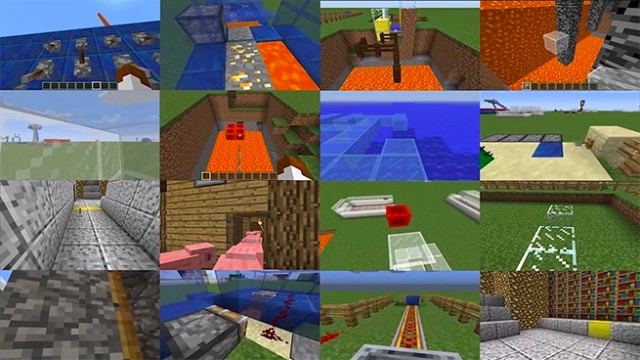
\includegraphics[width=0.4\textwidth]{Graphics/malmo-2.jpeg}
      \label{fig:malmo2}
    \end{subfigure}%
    \caption{Proyecto Malmo de Microsoft}
    \label{fig:malmo}
\end{figure}

La plataforma Malmo es una sofisticada plataforma de experimentación de IA construida sobre Minecraft, y diseñada para apoyar la investigación fundamental en inteligencia artificial.

La plataforma del Proyecto Malmo consiste en un mod para la versión Java, y un código que ayuda a los agentes de inteligencia artificial a percibir y actuar dentro del entorno de Minecraft. Los dos componentes pueden funcionar en Windows, Linux o Mac OS, y los investigadores pueden programar sus agentes en cualquier lenguaje de programación con el que se sientan cómodos.

Minecraft es ideal para la investigación de la inteligencia artificial por la misma razón por la que resulta adictivo para los millones de aficionados que entran en su mundo virtual cada día. A diferencia de otros juegos de ordenador, Minecraft ofrece a sus usuarios un sinfín de posibilidades, que van desde tareas sencillas, como caminar en busca de un tesoro, hasta otras complejas, como construir una estructura con un grupo de compañeros de equipo.

\subsubsection{MineRL y la prueba del Diamante}

Esta ambiciosa competición está diseñada para impulsar los avances en el aprendizaje de refuerzo con muestras eficientes y con prejuicios humanos. El aprendizaje eficiente por muestreo es un reto clave, ya que los algoritmos actuales suelen requerir millones de muestras para aprender a realizar tareas concretas, lo que limita el alcance y la aplicabilidad de estos enfoques. Esta competición se basa en una tarea compleja, en datos de demostración a gran escala y en una configuración de evaluación que requiere y premia el aprendizaje eficiente de las muestras y la generalización efectiva. (\cite{hofmann2019minecraft})

Comparando entre la inteligencia artificial y las capacidades mentales de un niño de siete años, apoyándonos en el popular videojuego Minecraft, donde dicho humano puede aprender a encontrar un diamante raro en el juego tras ver una rápida demostración en YouTube. La inteligencia artificial (IA) estaría lejos de lograrlo de esta forma. Pero a través de una competición informática los investigadores esperan reducir la distancia entre la máquina y el niño y, de este modo, se reduciría la potencia de cálculo necesaria para entrenar a las IA.
Los competidores pueden tardar hasta cuatro días y utilizar no más de ocho millones de pasos para entrenar a sus IA a encontrar un diamante. Eso es mucho más tiempo del que tardaría un niño en aprender, pero mucho más rápido que los modelos típicos de IA de hoy en día.

El concurso está diseñado para estimular los avances del aprendizaje por imitación que contrasta con la técnica de aprendizaje por refuerzo. El concurso se centra en el uso de la imitación para arrancar el aprendizaje, de modo que las IA no tengan que dedicar tanto tiempo a explorar el entorno para averiguar lo que es posible a partir de los primeros principios, y en su lugar utilicen los conocimientos que los humanos han acumulado. 

Para llegar al tesoro del diamante, los jugadores controlados por la IA, o agentes, en el concurso MineRL tienen que dominar un proceso de varios pasos. Primero, recogen madera y hierro para fabricar picos. Luego construyen antorchas para iluminar el camino. También pueden llevar un cubo de agua para apagar las corrientes de lava subterráneas. Una vez preparado todo eso, una IA puede empezar a explorar pozos mineros y cuevas, así como a hacer túneles bajo tierra para buscar mineral de diamante.

Para crear datos de entrenamiento para la competición, los organizadores de MineRL crearon un servidor público de Minecraft y reclutaron a personas para que completaran retos diseñados para demostrar tareas específicas, como la elaboración de diversas herramientas. Al final, capturaron 60 millones de ejemplos de acciones que podían realizarse en una situación determinada y aproximadamente 1.000 horas de comportamiento grabado para entregar a los equipos. Las grabaciones representan uno de los primeros y mayores conjuntos de datos dedicados específicamente a la investigación del aprendizaje por imitación.

\section{Abstraction and Reasoning Corpus (ARC)}\label{section:state-of-the-art:arc}

\begin{figure}[ht!]
    \centering
    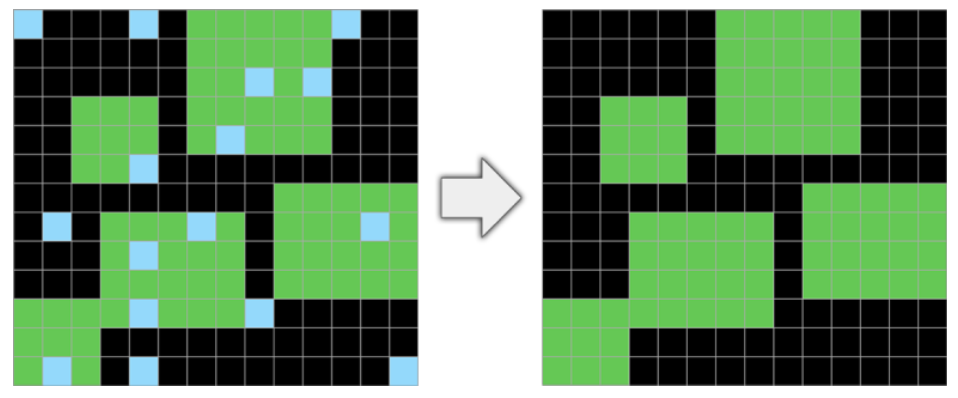
\includegraphics[width=0.7\textwidth]{Graphics/arc-2.png}
    \caption{Tarea de eliminar el ruido.}
    \label{fig:arc-1}
\end{figure}

\begin{figure}[ht!]
    \centering
    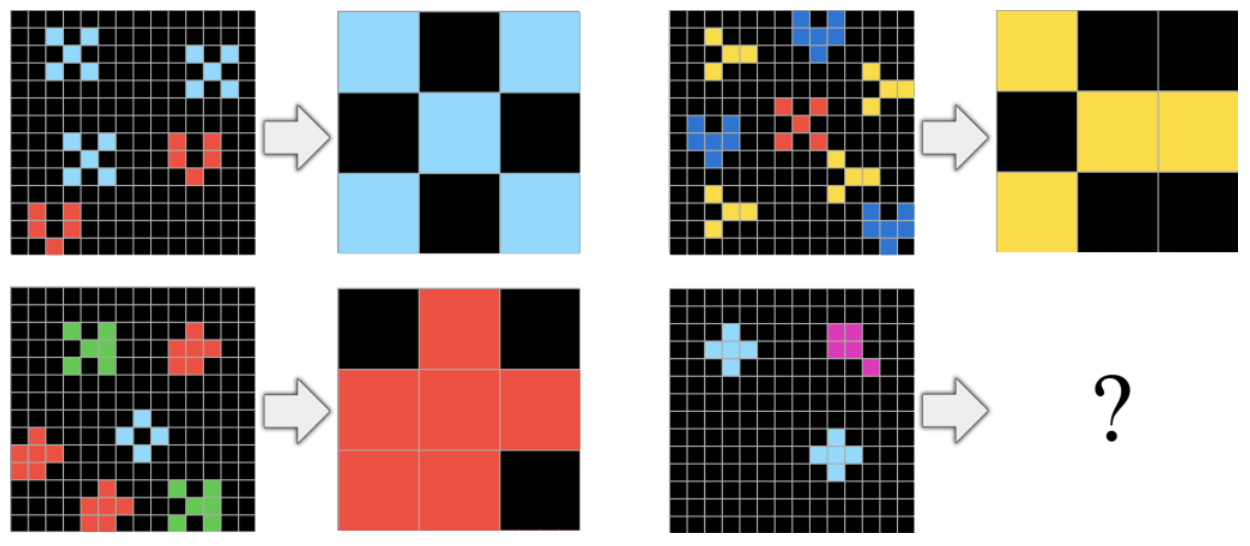
\includegraphics[width=0.7\textwidth]{Graphics/arc-1.png}
    \caption{Tarea de encontrar la figura que más se repite.}
    \label{fig:arc-2}
\end{figure}

\begin{figure}[ht!]
    \centering
    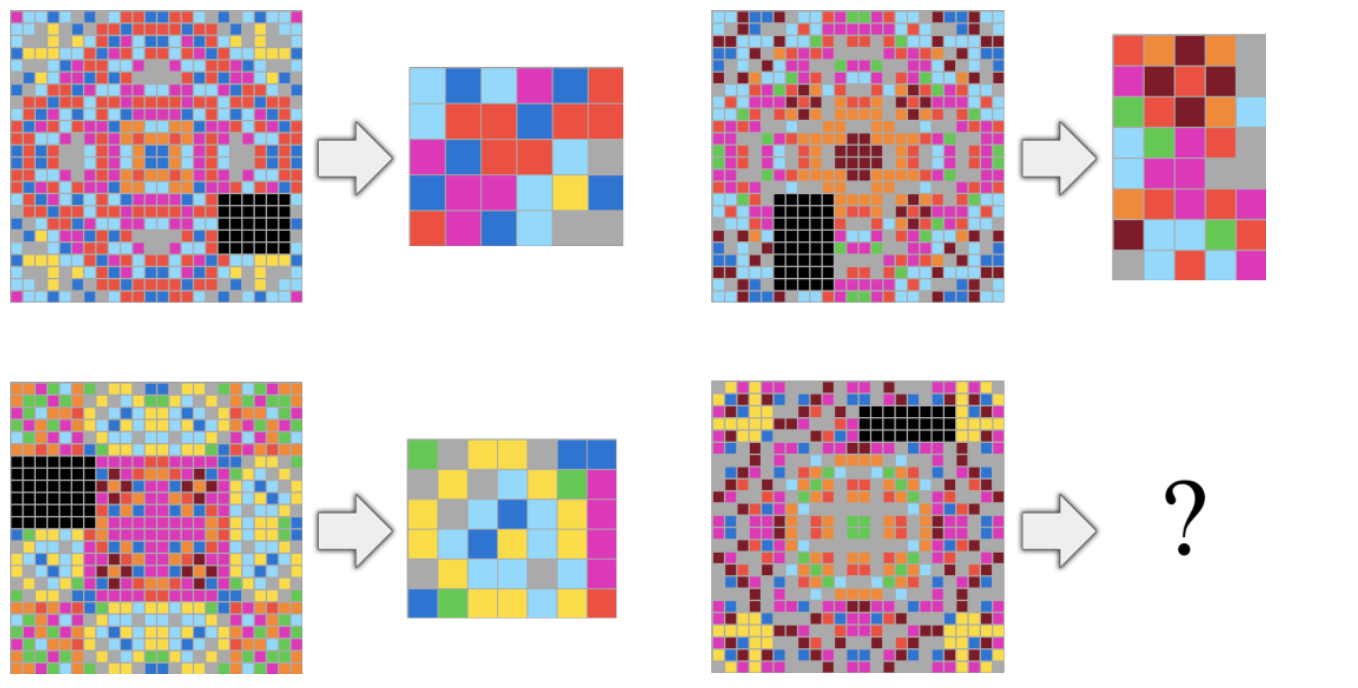
\includegraphics[width=0.7\textwidth]{Graphics/arc-3.png}
    \caption{Tarea de completar la imagen.}
    \label{fig:arc-3}
\end{figure}

El ARC puede considerarse como una referencia de inteligencia artificial general, como una referencia de síntesis de programas o como una prueba de inteligencia psicométrica. Está dirigido tanto a los humanos como a los sistemas de inteligencia artificial que pretenden emular una forma de inteligencia fluida general similar a la humana al mantenerse cerca del formato de los test psicométricos de inteligencia. 

Se centra en la medición de la generalización consciente del desarrollador, en lugar de la agilidad específica para la tarea, presentando únicamente tareas novedosas en el conjunto de evaluación. Las tareas presentadas son abstractas y deben ser comprendidas por el examinador con pocos ejemplos. En ARC se controla cuantitativamente la experiencia proporcionando sólo una cantidad fija de datos de entrenamiento para cada tarea y presentando sólo las tareas que no se prestan a la generación artificial de nuevos datos, obligando así a la eficiencia de los algoritmos a captar la esencia de la habilidad que se requiere.

Enumera explícitamente el conjunto completo de preconceptos como se propone en (\ref{section:state-of-the-art:a-good-measure-of-inteligence}), y permite una comparación de inteligencia general justa entre humanos y máquinas al requerir únicamente preconceptos cercanos al conocimiento previo humano innato. Tales como contar, nociones topográficas para la forma, tamaño, posición y color; nociones de la interacción entre objetos entre otras.

ARC comprende un conjunto de entrenamiento y un conjunto de evaluación. El conjunto de entrenamiento incluye 400 tareas, mientras que el conjunto de evaluación incluye 600 tareas. El conjunto de evaluación se divide a su vez en un conjunto de evaluación público (400 tareas) y un conjunto de evaluación privado (200 tareas). Cada tarea consta de un pequeño número de ejemplos de demostración (3,3 de media), y un pequeño número de ejemplos de prueba (generalmente 1, aunque puede ser 2 o 3 en casos raros). Cada ejemplo consta de una cuadrícula de entrada y una cuadrícula de salida. Cada cuadrícula es una cuadrícula literal de símbolos (cada símbolo se visualiza normalmente a través de un color único), como se ve en la figura \ref{fig:arc-2}. Hay 10 símbolos (o colores) únicos. Una cuadrícula puede tener cualquier altura o anchura entre 1x1 y 30x30, ambos inclusive (la altura media es 9 y la anchura media es 10).

El ARC sólo evalúa una forma general de inteligencia fluida, centrada en el razonamiento y la abstracción. El ARC no incluye el lenguaje, las imágenes de objetos del mundo real ni el sentido común del mundo real. El ARC busca sólo

\section{Discución}

Se han repasado los entornos de evaluación para algoritmos de aprendizaje por refuerzo, comenzando por aquellos que emplean juegos estáticos con tareas conocidas, luego evolucionando a problemas más complejos y con la capacidad de generar proceduralmente sus niveles para evitar sobreajuste. Terminando en entornos de evaluación que toman en cuentas tareas abstractas como las presentadas en MineRL y la toma de principios de la inteligencia animal en la busqueda de lo innato. Todos buscando evaluar sistemas con capacidades de generalización amplia pero sin concebirse para los que tienen inteligencia similar a la humana o presentar fundamentos para la validación de su evaluación en la búsqueda de inteligencia.

El ARC tiene buenos aspectos para destacar y cumple con un gran número características de un buen evaluador de inteligencia. Aún así su ámbito de habilidad se centra en sistemas inteligentes estáticos de entrada-salida, sin oportunidad de interacción con el entorno más allá de los ejemplos. Las tareas se crean manualmente por lo que son fijas, no generativas. También se hace complejo evaluar a los algoritmos de aprendizaje por reforzamiento dado la forma en que está diseñada la prueba. Las tareas de propósito general capturadas en ARC carecen del concepto de tiempo. Las nociones de topología se deben dar de forma implícita. 

Es necesario y más justo replantear las premisas teniendo en cuenta el efecto del tiempo en la dinámica del entorno, la percepción explícita de los cambios topográficos y los efectos acción-reacción. Llevar las tareas a conceptos más primitivos en términos de aprendizaje sin descuidar la dificultad de generalización. Y modelar un modelo de evaluación que aplique para agentes inteligentes como a humanos. Por estos motivos en el siguiente capítulo se propone la creación un entorno que cumpla con estos paradigmas: El \textit{Universal test for humans or inteligen agents (UTHOPIA)}.